\documentclass{article}
\usepackage{tikz}

\begin{document}

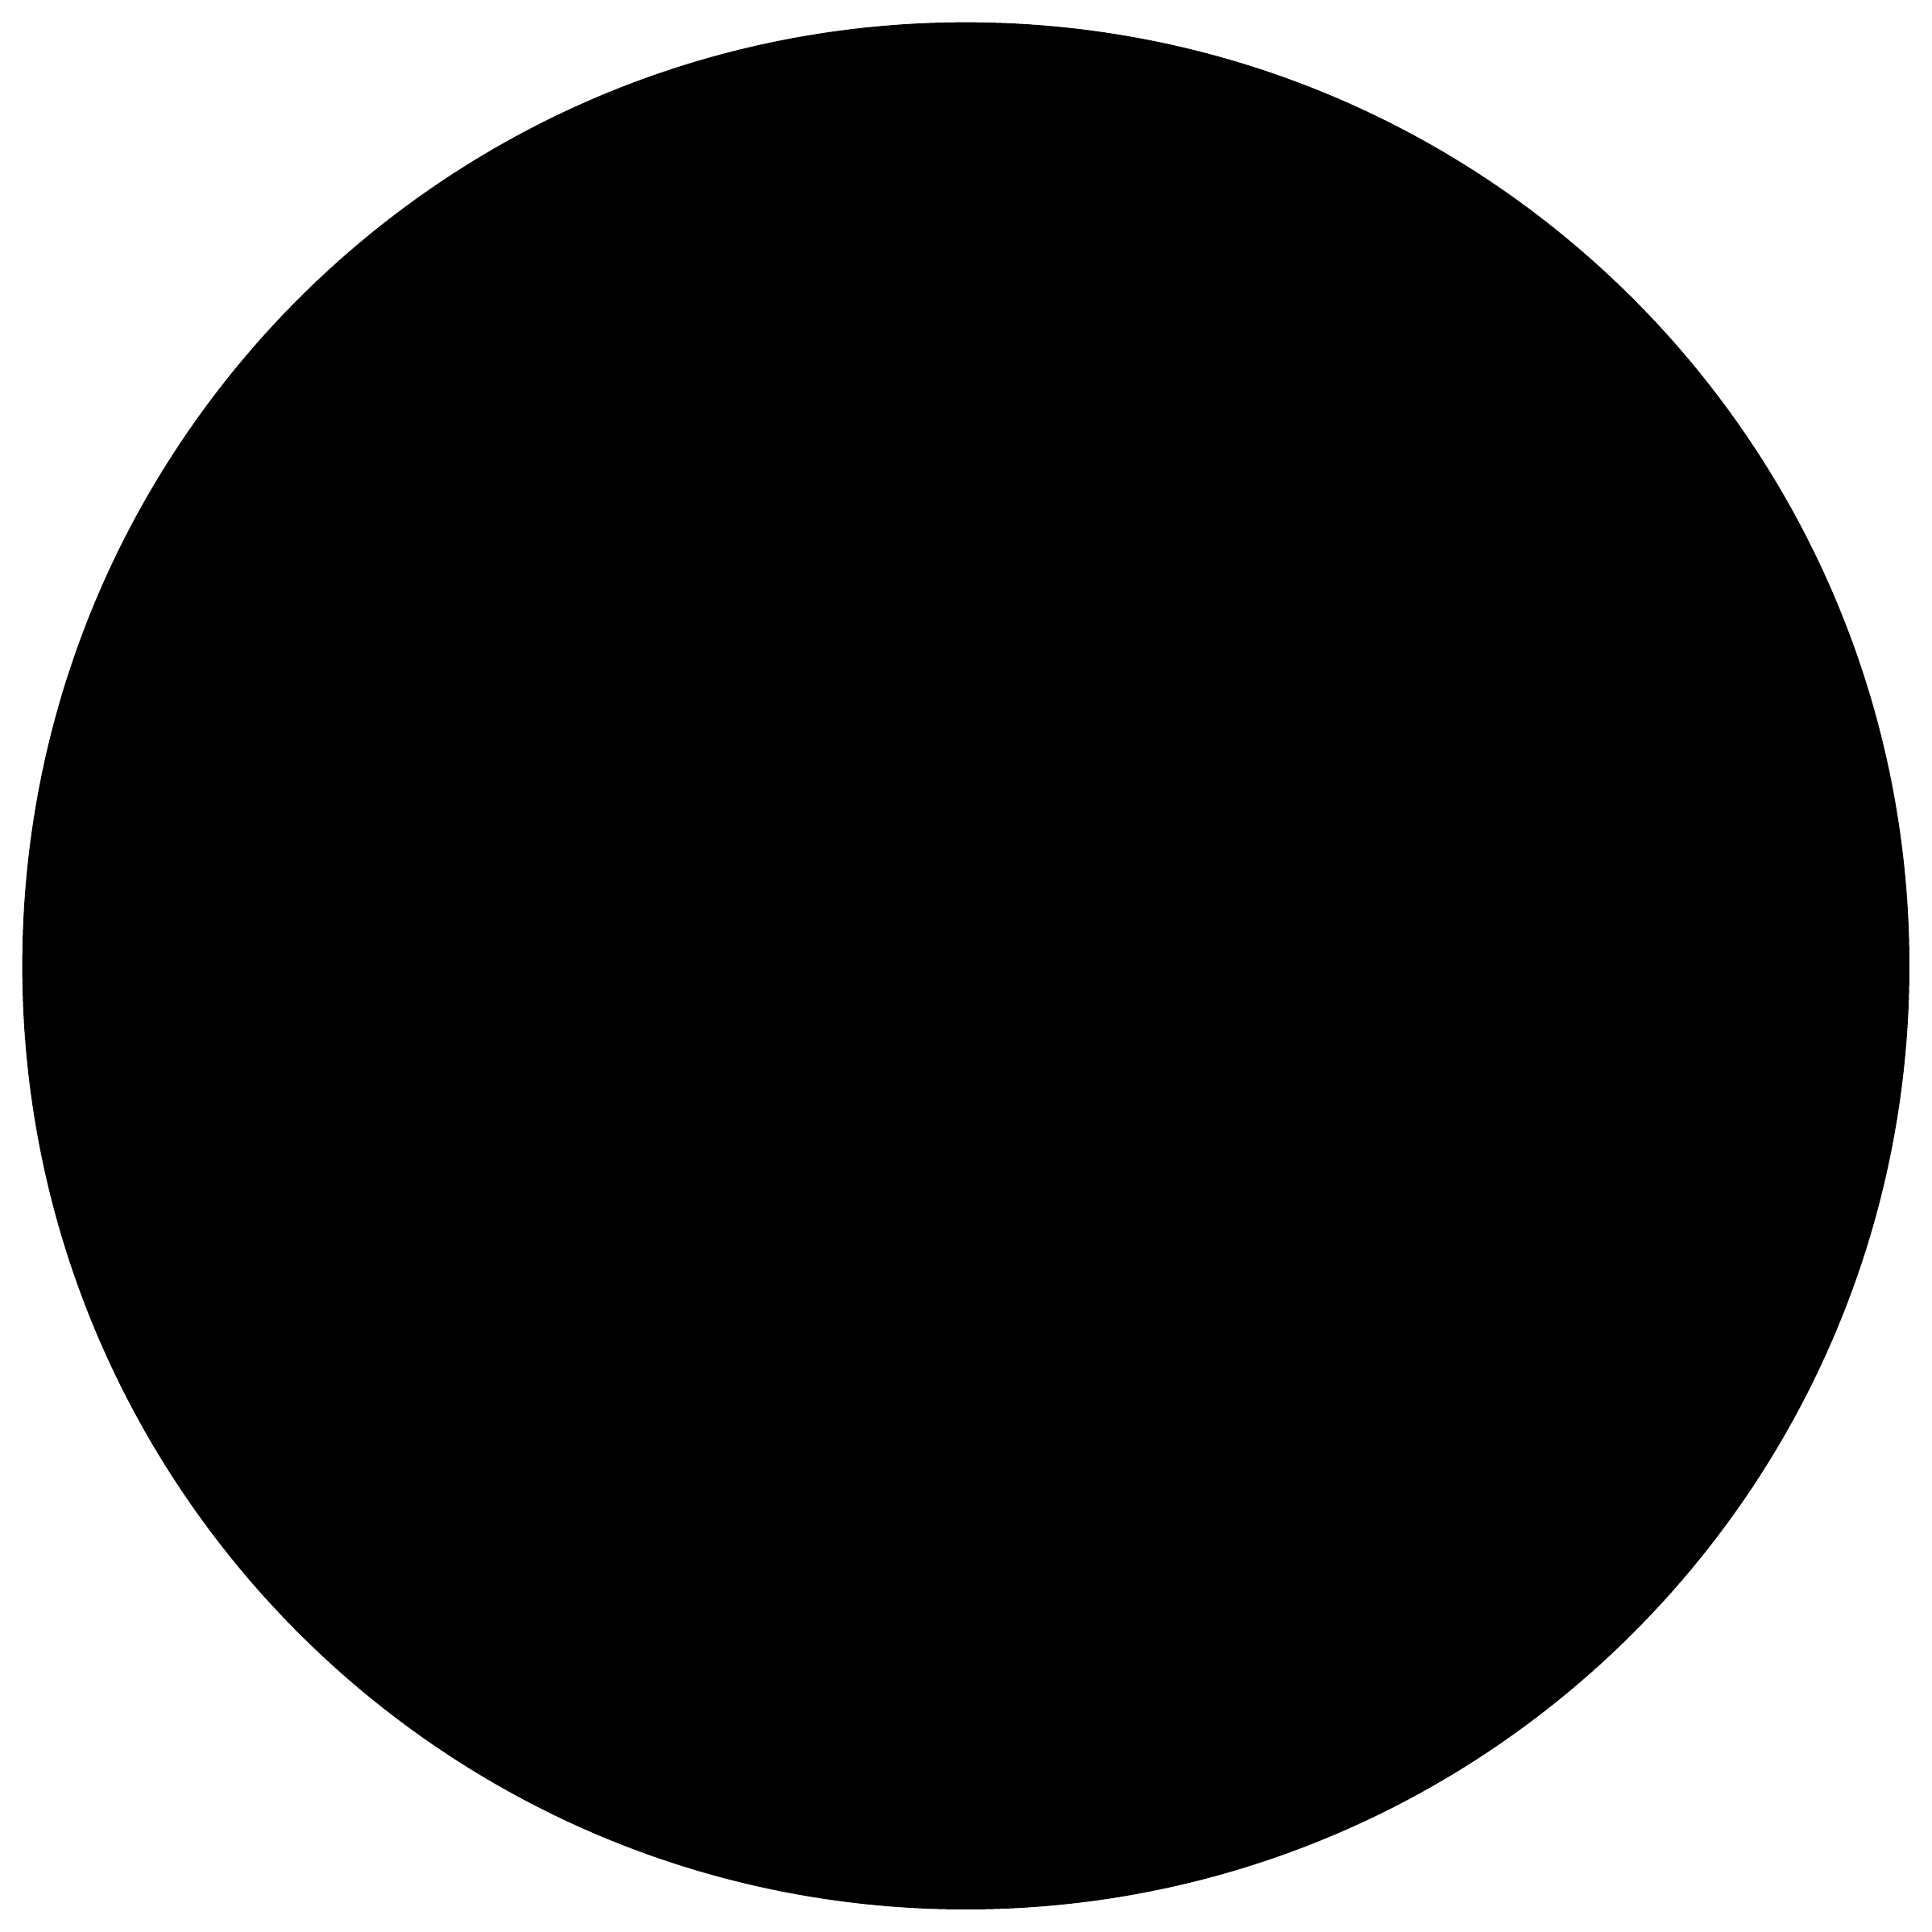
\begin{tikzpicture}[scale=1.5, every node/.style={circle, fill, inner sep=0pt, minimum size=6pt}]

% Define colors for nodes
\definecolor{blueNode}{RGB}{0, 128, 255}
\definecolor{redNode}{RGB}{255, 0, 0}
\definecolor{greenNode}{RGB}{0, 128, 0}

% Create nodes
\node[blueNode] (a) at (-2, -1) {};
\node[redNode] (b) at (-2, 1) {};
\node[greenNode] (c) at (-1, -1) {};
\node[redNode] (d) at (0, 2) {};
\node[blueNode] (e) at (1, -1) {};
\node[blueNode] (f) at (2, -1) {};

% Draw edges
\draw (a) -- (b);
\draw (b) -- (d);
\draw (c) -- (d);
\draw (d) -- (e);
\draw (d) -- (f);
\draw (e) -- (f);

% Second diagram
\begin{scope}[xshift=3cm]
\node[blueNode] (a') at (-2, -1) {};
\node[redNode] (b') at (-2, 1) {};
\node[greenNode] (c') at (-1, -1) {};
\node[blueNode] (d') at (0, 2) {};
\node[redNode] (e') at (1, -1) {};
\node[greenNode] (f') at (2, -1) {};

\draw (a') -- (b');
\draw (b') -- (d');
\draw (c') -- (d');
\draw (d') -- (e');
\draw (d') -- (f');
\draw (e') -- (f');
\end{scope}

% Third diagram
\begin{scope}[xshift=6cm]
\node[blueNode] (a'') at (-2, -1) {};
\node[redNode] (b'') at (-2, 1) {};
\node[greenNode] (c'') at (-1, -1) {};
\node[redNode] (d'') at (0, 2) {};
\node[blueNode] (e'') at (1, -1) {};
\node[blueNode] (f'') at (2, -1) {};

\draw (a'') -- (b'');
\draw (b'') -- (d'');
\draw (c'') -- (d'');
\draw (d'') -- (e'');
\draw (d'') -- (f'');
\draw (e'') -- (f'');
\end{scope}

% Description
\begin{scope}[yshift=-2.5cm]
\node at (0, -1.5) {\textbf{\large Maximal case (up to isomorphism) where $u$ and $v$ do not have a common neighbor and $G$ has a triangle. Even this maximal case is $3$-colorable.}};
\end{scope}

\end{tikzpicture}

\end{document}